% =====================================================================
%  pysic-rs: A Validated Mathematical-Physics Engine in Rust
%  arXiv preprint — HFThot Research Lab
%  Compile: pdflatex -interaction=nonstopmode pysic_rs_arxiv.tex  (x2)
% =====================================================================
\documentclass[11pt,a4paper]{article}

\usepackage[T1]{fontenc}
\usepackage[utf8]{inputenc}
\usepackage{lmodern}
\usepackage{microtype}
\usepackage{geometry}
\geometry{a4paper, left=2.6cm, right=2.6cm, top=2.6cm, bottom=2.6cm}
\usepackage{amsmath,amssymb,amsthm,mathtools,bm}
\usepackage{booktabs}
\usepackage{xcolor}
\usepackage{tcolorbox}
\tcbuselibrary{skins,breakable}
\usepackage{tikz}
\usepackage{pgfplots}
\pgfplotsset{compat=1.18}
\usetikzlibrary{positioning,arrows.meta,fit,backgrounds,calc}
\usepackage{listings}
\usepackage{caption}
\usepackage[numbers,sort&compress]{natbib}
\usepackage{hyperref}
\hypersetup{colorlinks=true,linkcolor=blue!50!black,citecolor=blue!50!black,urlcolor=blue!60!black}

\definecolor{rustorange}{RGB}{206,102,0}
\definecolor{teal}{RGB}{42,157,143}
\definecolor{gold}{RGB}{201,162,39}
\definecolor{softred}{RGB}{192,57,43}

\lstdefinelanguage{Rust}{
  morekeywords={as,break,const,continue,crate,dyn,else,enum,extern,false,fn,for,
    if,impl,in,let,loop,match,mod,move,mut,pub,ref,return,self,Self,static,struct,
    super,trait,true,type,unsafe,use,where,while,f64,usize,i32,bool,Vec,Option,Result},
  sensitive=true,
  morecomment=[l]{//}, morecomment=[s]{/*}{*/},
  morestring=[b]", morestring=[b]',
}
\lstset{
  basicstyle=\ttfamily\footnotesize,
  keywordstyle=\color{rustorange}\bfseries,
  commentstyle=\color{gray}\itshape,
  stringstyle=\color{teal},
  breaklines=true, frame=single, rulecolor=\color{gray!40},
  backgroundcolor=\color{gray!4}, showstringspaces=false,
  xleftmargin=8pt, framexleftmargin=8pt,
}

\newtcolorbox{lesson}{colback=gold!6!white,colframe=gold!70!black,
  title=\textbf{Lesson},fonttitle=\small\bfseries,breakable}
\newtcolorbox{pitfall}{colback=softred!5!white,colframe=softred!65!black,
  title=\textbf{Failure mode},fonttitle=\small\bfseries,breakable}

\theoremstyle{plain}
\newtheorem{theorem}{Theorem}[section]
\newtheorem{proposition}[theorem]{Proposition}
\theoremstyle{definition}
\newtheorem{definition}[theorem]{Definition}
\newtheorem{remark}[theorem]{Remark}

\newcommand{\datadiracnorm}{(10,2.3802e-15) (50,1.4782e-14) (100,3.0818e-14) (500,1.4256e-13) (1000,2.8137e-13) (5000,1.4449e-12)}
\newcommand{\databoxconv}{(50,3.1617e-04) (100,8.0624e-05) (200,2.0357e-05) (400,5.1148e-06) (800,1.2819e-06)}
\newcommand{\databesseljzero}{(0.000,1.00000) (0.101,0.99748) (0.201,0.98992) (0.302,0.97740) (0.402,0.96000) (0.503,0.93786) (0.603,0.91114) (0.704,0.88004) (0.804,0.84480) (0.905,0.80568) (1.005,0.76298) (1.106,0.71701) (1.206,0.66812) (1.307,0.61667) (1.407,0.56304) (1.508,0.50762) (1.608,0.45082) (1.709,0.39305) (1.809,0.33473) (1.910,0.27627) (2.010,0.21810) (2.111,0.16062) (2.211,0.10422) (2.312,0.04931) (2.412,-0.00375) (2.513,-0.05461) (2.613,-0.10293) (2.714,-0.14841) (2.814,-0.19077) (2.915,-0.22974) (3.015,-0.26512) (3.116,-0.29670) (3.216,-0.32434) (3.317,-0.34790) (3.417,-0.36730) (3.518,-0.38248) (3.618,-0.39343) (3.719,-0.40016) (3.819,-0.40273) (3.920,-0.40122) (4.020,-0.39575) (4.121,-0.38647) (4.221,-0.37355) (4.322,-0.35722) (4.422,-0.33770) (4.523,-0.31525) (4.623,-0.29014) (4.724,-0.26268) (4.824,-0.23317) (4.925,-0.20195) (5.025,-0.16933) (5.126,-0.13567) (5.226,-0.10131) (5.327,-0.06659) (5.427,-0.03185) (5.528,0.00257) (5.628,0.03634) (5.729,0.06916) (5.829,0.10070) (5.930,0.13071) (6.030,0.15890) (6.131,0.18503) (6.231,0.20889) (6.332,0.23027) (6.432,0.24901) (6.533,0.26497) (6.633,0.27803) (6.734,0.28810) (6.834,0.29515) (6.935,0.29913) (7.035,0.30006) (7.136,0.29797) (7.236,0.29292) (7.337,0.28500) (7.437,0.27434) (7.538,0.26107) (7.638,0.24535) (7.739,0.22739) (7.839,0.20737) (7.940,0.18553) (8.040,0.16211) (8.141,0.13734) (8.241,0.11151) (8.342,0.08487) (8.442,0.05770) (8.543,0.03027) (8.643,0.00286) (8.744,-0.02427) (8.844,-0.05084) (8.945,-0.07660) (9.045,-0.10130) (9.146,-0.12472) (9.246,-0.14662) (9.347,-0.16682) (9.447,-0.18513) (9.548,-0.20138) (9.648,-0.21545) (9.749,-0.22720) (9.849,-0.23655) (9.950,-0.24344) (10.050,-0.24780) (10.151,-0.24964) (10.251,-0.24895) (10.352,-0.24577) (10.452,-0.24015) (10.553,-0.23217) (10.653,-0.22194) (10.754,-0.20957) (10.854,-0.19521) (10.955,-0.17902) (11.055,-0.16119) (11.156,-0.14189) (11.256,-0.12134) (11.357,-0.09976) (11.457,-0.07736) (11.558,-0.05438) (11.658,-0.03106) (11.759,-0.00762) (11.859,0.01569) (11.960,0.03866) (12.060,0.06104) (12.161,0.08262) (12.261,0.10319) (12.362,0.12256) (12.462,0.14053) (12.563,0.15696) (12.663,0.17167) (12.764,0.18454) (12.864,0.19546) (12.965,0.20432) (13.065,0.21106) (13.166,0.21563) (13.266,0.21800) (13.367,0.21816) (13.467,0.21612) (13.568,0.21192) (13.668,0.20563) (13.769,0.19731) (13.869,0.18707) (13.970,0.17502) (14.070,0.16130) (14.171,0.14605) (14.271,0.12945) (14.372,0.11165) (14.472,0.09286) (14.573,0.07327) (14.673,0.05307) (14.774,0.03248) (14.874,0.01170) (14.975,-0.00906) (15.075,-0.02959) (15.176,-0.04968) (15.276,-0.06915) (15.377,-0.08779) (15.477,-0.10542) (15.578,-0.12188) (15.678,-0.13701) (15.779,-0.15066) (15.879,-0.16271) (15.980,-0.17305) (16.080,-0.18158) (16.181,-0.18823) (16.281,-0.19295) (16.382,-0.19569) (16.482,-0.19645) (16.583,-0.19523) (16.683,-0.19205) (16.784,-0.18696) (16.884,-0.18002) (16.985,-0.17131) (17.085,-0.16092) (17.186,-0.14898) (17.286,-0.13561) (17.387,-0.12095) (17.487,-0.10516) (17.588,-0.08840) (17.688,-0.07084) (17.789,-0.05267) (17.889,-0.03408) (17.990,-0.01525) (18.090,0.00364) (18.191,0.02238) (18.291,0.04079) (18.392,0.05869) (18.492,0.07591) (18.593,0.09226) (18.693,0.10760) (18.794,0.12178) (18.894,0.13465) (18.995,0.14610) (19.095,0.15601) (19.196,0.16431) (19.296,0.17091) (19.397,0.17575) (19.497,0.17880) (19.598,0.18003) (19.698,0.17945) (19.799,0.17706) (19.899,0.17290) (20.000,0.16702)}
\newcommand{\databesselenv}{(0.101,2.51682) (0.201,1.77966) (0.302,1.45308) (0.402,1.25841) (0.503,1.12555) (0.603,1.02749) (0.704,0.95127) (0.804,0.88983) (0.905,0.83894) (1.005,0.79589) (1.106,0.75885) (1.206,0.72654) (1.307,0.69804) (1.407,0.67265) (1.508,0.64984) (1.608,0.62920) (1.709,0.61042) (1.809,0.59322) (1.910,0.57740) (2.010,0.56278) (2.111,0.54921) (2.211,0.53659) (2.312,0.52479) (2.412,0.51374) (2.513,0.50336) (2.613,0.49359) (2.714,0.48436) (2.814,0.47563) (2.915,0.46736) (3.015,0.45951) (3.116,0.45203) (3.216,0.44491) (3.317,0.43812) (3.417,0.43163) (3.518,0.42542) (3.618,0.41947) (3.719,0.41376) (3.819,0.40828) (3.920,0.40301) (4.020,0.39794) (4.121,0.39306) (4.221,0.38835) (4.322,0.38381) (4.422,0.37942) (4.523,0.37518) (4.623,0.37108) (4.724,0.36712) (4.824,0.36327) (4.925,0.35955) (5.025,0.35593) (5.126,0.35242) (5.226,0.34902) (5.327,0.34571) (5.427,0.34250) (5.528,0.33937) (5.628,0.33632) (5.729,0.33336) (5.829,0.33047) (5.930,0.32766) (6.030,0.32492) (6.131,0.32225) (6.231,0.31964) (6.332,0.31709) (6.432,0.31460) (6.533,0.31217) (6.633,0.30980) (6.734,0.30748) (6.834,0.30521) (6.935,0.30299) (7.035,0.30082) (7.136,0.29869) (7.236,0.29661) (7.337,0.29457) (7.437,0.29257) (7.538,0.29062) (7.638,0.28870) (7.739,0.28682) (7.839,0.28497) (7.940,0.28316) (8.040,0.28139) (8.141,0.27965) (8.241,0.27794) (8.342,0.27626) (8.442,0.27461) (8.543,0.27299) (8.643,0.27140) (8.744,0.26983) (8.844,0.26829) (8.945,0.26678) (9.045,0.26530) (9.146,0.26383) (9.246,0.26240) (9.347,0.26098) (9.447,0.25959) (9.548,0.25822) (9.648,0.25687) (9.749,0.25554) (9.849,0.25424) (9.950,0.25295) (10.050,0.25168) (10.151,0.25043) (10.251,0.24920) (10.352,0.24799) (10.452,0.24679) (10.553,0.24562) (10.653,0.24445) (10.754,0.24331) (10.854,0.24218) (10.955,0.24107) (11.055,0.23997) (11.156,0.23889) (11.256,0.23782) (11.357,0.23676) (11.457,0.23572) (11.558,0.23469) (11.658,0.23368) (11.759,0.23268) (11.859,0.23169) (11.960,0.23072) (12.060,0.22975) (12.161,0.22880) (12.261,0.22786) (12.362,0.22693) (12.462,0.22602) (12.563,0.22511) (12.663,0.22422) (12.764,0.22333) (12.864,0.22246) (12.965,0.22159) (13.065,0.22074) (13.166,0.21990) (13.266,0.21906) (13.367,0.21824) (13.467,0.21742) (13.568,0.21661) (13.668,0.21582) (13.769,0.21503) (13.869,0.21425) (13.970,0.21347) (14.070,0.21271) (14.171,0.21195) (14.271,0.21121) (14.372,0.21047) (14.472,0.20973) (14.573,0.20901) (14.673,0.20829) (14.774,0.20758) (14.874,0.20688) (14.975,0.20619) (15.075,0.20550) (15.176,0.20482) (15.276,0.20414) (15.377,0.20347) (15.477,0.20281) (15.578,0.20216) (15.678,0.20151) (15.779,0.20086) (15.879,0.20023) (15.980,0.19960) (16.080,0.19897) (16.181,0.19835) (16.281,0.19774) (16.382,0.19713) (16.482,0.19653) (16.583,0.19593) (16.683,0.19534) (16.784,0.19476) (16.884,0.19418) (16.985,0.19360) (17.085,0.19303) (17.186,0.19247) (17.286,0.19191) (17.387,0.19135) (17.487,0.19080) (17.588,0.19025) (17.688,0.18971) (17.789,0.18918) (17.889,0.18864) (17.990,0.18812) (18.090,0.18759) (18.191,0.18707) (18.291,0.18656) (18.392,0.18605) (18.492,0.18554) (18.593,0.18504) (18.693,0.18454) (18.794,0.18405) (18.894,0.18356) (18.995,0.18307) (19.095,0.18259) (19.196,0.18211) (19.296,0.18164) (19.397,0.18116) (19.497,0.18070) (19.598,0.18023) (19.698,0.17977) (19.799,0.17932) (19.899,0.17886) (20.000,0.17841)}
\newcommand{\dataairy}{(-12.0000,-0.066555) (-11.9372,-0.001283) (-11.8745,0.064053) (-11.8117,0.126407) (-11.7490,0.182904) (-11.6862,0.230972) (-11.6234,0.268450) (-11.5607,0.293686) (-11.4979,0.305599) (-11.4351,0.303724) (-11.3724,0.288219) (-11.3096,0.259850) (-11.2469,0.219947) (-11.1841,0.170333) (-11.1213,0.113242) (-11.0586,0.051205) (-10.9958,-0.013057) (-10.9331,-0.076758) (-10.8703,-0.137168) (-10.8075,-0.191728) (-10.7448,-0.238157) (-10.6820,-0.274543) (-10.6192,-0.299419) (-10.5565,-0.311815) (-10.4937,-0.311291) (-10.4310,-0.297943) (-10.3682,-0.272394) (-10.3054,-0.235758) (-10.2427,-0.189581) (-10.1799,-0.135780) (-10.1172,-0.076550) (-10.0544,-0.014276) (-9.9916,0.048563) (-9.9289,0.109500) (-9.8661,0.166171) (-9.8033,0.216407) (-9.7406,0.258315) (-9.6778,0.290345) (-9.6151,0.311343) (-9.5523,0.320587) (-9.4895,0.317807) (-9.4268,0.303184) (-9.3640,0.277336) (-9.3013,0.241290) (-9.2385,0.196428) (-9.1757,0.144438) (-9.1130,0.087241) (-9.0502,0.026919) (-8.9874,-0.034362) (-8.9247,-0.094433) (-8.8619,-0.151196) (-8.7992,-0.202699) (-8.7364,-0.247198) (-8.6736,-0.283217) (-8.6109,-0.309589) (-8.5481,-0.325490) (-8.4854,-0.330462) (-8.4226,-0.324421) (-8.3598,-0.307645) (-8.2971,-0.280765) (-8.2343,-0.244733) (-8.1715,-0.200783) (-8.1088,-0.150386) (-8.0460,-0.095196) (-7.9833,-0.036994) (-7.9205,0.022370) (-7.8577,0.081041) (-7.7950,0.137212) (-7.7322,0.189184) (-7.6695,0.235409) (-7.6067,0.274543) (-7.5439,0.305473) (-7.4812,0.327348) (-7.4184,0.339602) (-7.3556,0.341957) (-7.2929,0.334427) (-7.2301,0.317314) (-7.1674,0.291183) (-7.1046,0.256850) (-7.0418,0.215344) (-6.9791,0.167877) (-6.9163,0.115804) (-6.8536,0.060580) (-6.7908,0.003722) (-6.7280,-0.053237) (-6.6653,-0.108791) (-6.6025,-0.161497) (-6.5397,-0.210014) (-6.4770,-0.253135) (-6.4142,-0.289813) (-6.3515,-0.319185) (-6.2887,-0.340589) (-6.2259,-0.353575) (-6.1632,-0.357908) (-6.1004,-0.353569) (-6.0377,-0.340751) (-5.9749,-0.319845) (-5.9121,-0.291424) (-5.8494,-0.256229) (-5.7866,-0.215140) (-5.7238,-0.169154) (-5.6611,-0.119360) (-5.5983,-0.066908) (-5.5356,-0.012980) (-5.4728,0.041233) (-5.4100,0.094560) (-5.3473,0.145878) (-5.2845,0.194131) (-5.2218,0.238352) (-5.1590,0.277681) (-5.0962,0.311377) (-5.0335,0.338835) (-4.9707,0.359587) (-4.9079,0.373310) (-4.8452,0.379829) (-4.7824,0.379109) (-4.7197,0.371260) (-4.6569,0.356518) (-4.5941,0.335246) (-4.5314,0.307916) (-4.4686,0.275096) (-4.4059,0.237439) (-4.3431,0.195667) (-4.2803,0.150550) (-4.2176,0.102896) (-4.1548,0.053533) (-4.0921,0.003293) (-4.0293,-0.047002) (-3.9665,-0.096553) (-3.9038,-0.144601) (-3.8410,-0.190429) (-3.7782,-0.233382) (-3.7155,-0.272868) (-3.6527,-0.308366) (-3.5900,-0.339435) (-3.5272,-0.365710) (-3.4644,-0.386911) (-3.4017,-0.402839) (-3.3389,-0.413376) (-3.2762,-0.418482) (-3.2134,-0.418194) (-3.1506,-0.412618) (-3.0879,-0.401926) (-3.0251,-0.386350) (-2.9623,-0.366174) (-2.8996,-0.341729) (-2.8368,-0.313383) (-2.7741,-0.281537) (-2.7113,-0.246616) (-2.6485,-0.209063) (-2.5858,-0.169328) (-2.5230,-0.127869) (-2.4603,-0.085138) (-2.3975,-0.041581) (-2.3347,0.002370) (-2.2720,0.046301) (-2.2092,0.089820) (-2.1464,0.132559) (-2.0837,0.174181) (-2.0209,0.214375) (-1.9582,0.252866) (-1.8954,0.289409) (-1.8326,0.323794) (-1.7699,0.355845) (-1.7071,0.385417) (-1.6444,0.412400) (-1.5816,0.436715) (-1.5188,0.458312) (-1.4561,0.477168) (-1.3933,0.493290) (-1.3305,0.506707) (-1.2678,0.517469) (-1.2050,0.525649) (-1.1423,0.531335) (-1.0795,0.534631) (-1.0167,0.535656) (-0.9540,0.534535) (-0.8912,0.531406) (-0.8285,0.526413) (-0.7657,0.519701) (-0.7029,0.511422) (-0.6402,0.501728) (-0.5774,0.490768) (-0.5146,0.478691) (-0.4519,0.465644) (-0.3891,0.451767) (-0.3264,0.437197) (-0.2636,0.422065) (-0.2008,0.406494) (-0.1381,0.390601) (-0.0753,0.374495) (-0.0126,0.358277) (0.0502,0.342040) (0.1130,0.325871) (0.1757,0.309846) (0.2385,0.294034) (0.3013,0.278499) (0.3640,0.263293) (0.4268,0.248464) (0.4895,0.234053) (0.5523,0.220092) (0.6151,0.206609) (0.6778,0.193627) (0.7406,0.181161) (0.8033,0.169223) (0.8661,0.157820) (0.9289,0.146956) (0.9916,0.136629) (1.0544,0.126835) (1.1172,0.117568) (1.1799,0.108818) (1.2427,0.100574) (1.3054,0.092822) (1.3682,0.085547) (1.4310,0.078733) (1.4937,0.072363) (1.5565,0.066418) (1.6192,0.060881) (1.6820,0.055732) (1.7448,0.050952) (1.8075,0.046523) (1.8703,0.042424) (1.9331,0.038638) (1.9958,0.035147) (2.0586,0.031932) (2.1213,0.028975) (2.1841,0.026261) (2.2469,0.023773) (2.3096,0.021496) (2.3724,0.019414) (2.4351,0.017513) (2.4979,0.015781) (2.5607,0.014204) (2.6234,0.012770) (2.6862,0.011468) (2.7490,0.010288) (2.8117,0.009219) (2.8745,0.008252) (2.9372,0.007379) (3.0000,0.006591)}
\newcommand{\datazetaerr}{(1.050,3.452e-16) (1.123,1.000e-17) (1.197,3.134e-16) (1.270,2.069e-16) (1.344,3.797e-16) (1.417,4.438e-16) (1.491,3.353e-16) (1.564,3.719e-16) (1.638,2.029e-16) (1.711,4.371e-16) (1.785,3.496e-16) (1.858,6.165e-16) (1.932,1.000e-17) (2.005,1.354e-16) (2.079,1.408e-16) (2.152,1.459e-16) (2.226,4.518e-16) (2.299,3.100e-16) (2.373,1.591e-16) (2.446,4.887e-16) (2.520,4.994e-16) (2.593,1.698e-16) (2.667,6.916e-16) (2.740,8.791e-16) (2.814,3.571e-16) (2.887,1.811e-16) (2.961,5.505e-16) (3.034,3.715e-16) (3.108,7.514e-16) (3.181,1.898e-16) (3.255,3.833e-16) (3.328,7.736e-16) (3.402,1.000e-17) (3.475,3.931e-16) (3.549,1.980e-16) (3.622,1.000e-17) (3.696,2.006e-16) (3.769,8.073e-16) (3.843,2.030e-16) (3.916,1.000e-17) (3.990,2.050e-16) (4.063,1.000e-17) (4.137,2.068e-16) (4.210,2.077e-16) (4.284,2.085e-16) (4.357,4.184e-16) (4.431,4.198e-16) (4.504,2.106e-16) (4.578,4.224e-16) (4.651,2.118e-16) (4.724,1.062e-15) (4.798,1.000e-17) (4.871,4.267e-16) (4.945,1.069e-15) (5.018,1.000e-17) (5.092,4.293e-16) (5.165,1.290e-15) (5.239,2.154e-16) (5.312,6.473e-16) (5.386,2.161e-16) (5.459,2.164e-16) (5.533,1.084e-15) (5.606,6.510e-16) (5.680,6.518e-16) (5.753,1.088e-15) (5.827,4.355e-16) (5.900,8.719e-16) (5.974,2.182e-16) (6.047,2.184e-16) (6.121,2.186e-16) (6.194,4.375e-16) (6.268,1.000e-17) (6.341,1.000e-17) (6.415,6.577e-16) (6.488,1.000e-17) (6.562,6.586e-16) (6.635,1.000e-17) (6.709,1.000e-17) (6.782,2.199e-16) (6.856,6.600e-16) (6.929,4.402e-16) (7.003,2.202e-16) (7.076,6.609e-16) (7.150,2.204e-16) (7.223,6.614e-16) (7.297,2.206e-16) (7.370,2.206e-16) (7.444,2.207e-16) (7.517,4.415e-16) (7.591,4.417e-16) (7.664,2.209e-16) (7.738,2.210e-16) (7.811,1.000e-17) (7.885,6.632e-16) (7.958,2.211e-16) (8.032,1.000e-17) (8.105,6.636e-16) (8.179,6.638e-16) (8.252,1.000e-17) (8.326,1.000e-17) (8.399,6.641e-16) (8.472,2.214e-16) (8.546,2.214e-16) (8.619,1.000e-17) (8.693,8.860e-16) (8.766,8.861e-16) (8.840,4.431e-16) (8.913,2.216e-16) (8.987,4.432e-16) (9.060,2.216e-16) (9.134,4.433e-16) (9.207,4.433e-16) (9.281,4.434e-16) (9.354,8.868e-16) (9.428,4.434e-16) (9.501,4.435e-16) (9.575,6.652e-16) (9.648,2.218e-16) (9.722,2.218e-16) (9.795,2.218e-16) (9.869,4.436e-16) (9.942,1.000e-17) (10.016,4.437e-16) (10.089,4.437e-16) (10.163,2.218e-16) (10.236,1.000e-17) (10.310,2.219e-16) (10.383,2.219e-16) (10.457,1.000e-17) (10.530,1.000e-17) (10.604,4.438e-16) (10.677,2.219e-16) (10.751,4.438e-16) (10.824,8.877e-16) (10.898,2.219e-16) (10.971,6.658e-16) (11.045,2.219e-16) (11.118,4.439e-16) (11.192,4.439e-16) (11.265,2.220e-16) (11.339,2.220e-16) (11.412,4.439e-16) (11.486,4.439e-16) (11.559,2.220e-16) (11.633,2.220e-16) (11.706,2.220e-16) (11.780,4.440e-16) (11.853,2.220e-16) (11.927,2.220e-16) (12.000,2.220e-16)}
\newcommand{\dataadmH}{(0.25,0.375000) (0.5,1.500000) (1.0,6.000000) (1.5,13.500000) (2.0,24.000000) (2.5,37.500000) (3.0,54.000000)}
\newcommand{\dataricci}{(6,4.349e-08) (10,1.641e-08) (25,2.621e-09) (50,6.765e-10) (100,2.154e-10)}
\newcommand{\dataricciold}{(6,5.556e-02) (10,2.000e-02) (25,3.200e-03) (50,8.000e-04) (100,2.000e-04)}


\title{\textbf{pysic-rs}: A Validated Mathematical-Physics Engine in Rust,\\
and What Grading It Against Closed Forms Revealed}

\author{Melvin Alvarez\\
\small HFThot Research Lab\\
\small \texttt{contact@hfthot-lab.eu}}

\date{\today}

\begin{document}
\maketitle

\begin{abstract}
\noindent
We present \textbf{pysic-rs}, a CPU-only mathematical-physics library written in
Rust and exposed to Python through PyO3. It covers special functions, linear
algebra, ODE and PDE solvers, quantum mechanics, general relativity, gauge
theory, topology and electromagnetism, and is designed around a single
methodological commitment: every routine is \emph{graded} against a closed-form
result or a tabulated reference value, rather than demonstrated on a plot that
looks plausible.

We then report what applying that commitment uncovered. Preparing a pedagogical
walk-through of six equations connecting quantum mechanics to quantum gravity ---
Schr\"odinger, Dirac, Maxwell/Aharonov--Bohm, the ADM constraints and
Wheeler--DeWitt --- exposed \emph{eight} incorrect routines in the library's own
code, including a Dirac propagator whose norm grew to $3.6\times10^{57}$, an
eigensolver returning the matrix diagonal instead of its spectrum, Bessel
functions returning $+50.6$ for a quantity bounded by $1$, and a vacuum
spacetime reporting non-zero Ricci curvature.

The interesting content is not the bugs but their survival. We show that in
every case a test existed or could trivially have existed, and analyse why the
tests that were written could not have failed --- most starkly a Ricci-flatness
test that handed a \emph{constant} metric to a routine that differentiates its
argument, so that every derivative vanished and the invariant held trivially.
We argue that the discriminating property of a useful numerical test is not
coverage but \emph{falsifiability against an independently known quantity}, and
that oscillatory, unitary and gauge-invariant structures supply such quantities
almost for free.

All figures in this paper are generated from the library's own output. The
measured accuracies, the reproduction scripts and the companion notebook are
public.
\end{abstract}

\tableofcontents
\bigskip

% =====================================================================
\section{Introduction}

Scientific Python is typically a thin interpreted layer over a fast compiled
kernel. The compiled part is well tested; the interpreted part --- the loop over
modes, the boundary handling, the branch between a series and an asymptotic
expansion --- frequently is not. That layer is where the wall-clock time goes,
and it is also where silent numerical errors live, because it is the layer least
likely to be exercised against a known answer.

\textbf{pysic-rs} moves that layer into Rust. The performance argument is
routine and we do not belabour it. The argument we do want to make is about
correctness, and it has two parts.

\begin{enumerate}
\item \textbf{The type system removes a class of mistakes before run time.}
      Ownership and affine types eliminate use-after-free and data races;
      exhaustive matching eliminates unhandled branches; and the absence of
      implicit numeric coercion makes unit and index errors visible at compile
      time.
\item \textbf{The type system removes none of the mistakes we actually made.}
      Every defect reported in Section~\ref{sec:bugs} compiled cleanly, ran
      without panicking, and returned finite plausible-looking numbers. Types
      are necessary and radically insufficient.
\end{enumerate}

The second point is the subject of this paper. What caught these defects was not
the compiler and not code review, but the discipline of writing a document in
which every printed number had to be placed next to an independently known
value.

\subsection{Contributions}

\begin{itemize}
\item A description of the library's architecture and its validation
      discipline (Sections~\ref{sec:design}--\ref{sec:validation}).
\item The mathematical formulation of six equations it solves, each reduced to
      an invariant that a correct implementation must preserve exactly
      (Section~\ref{sec:physics}).
\item A post-mortem of eight defects, with an analysis of why the existing tests
      did not and structurally \emph{could} not detect them
      (Section~\ref{sec:bugs}).
\item Measured accuracy for the full special-function suite, replacing claims
      that were previously asserted (Section~\ref{sec:accuracy}).
\end{itemize}

% =====================================================================
\section{Design}\label{sec:design}

\subsection{Layering}

The crate is a pure-Rust core with an optional, feature-gated PyO3 binding
layer. Nothing in the core depends on Python, on BLAS or LAPACK, or on a GPU
runtime; the numerics are written out explicitly so that each algorithm's
branch structure is legible and testable in isolation.

\begin{figure}[h]
\centering
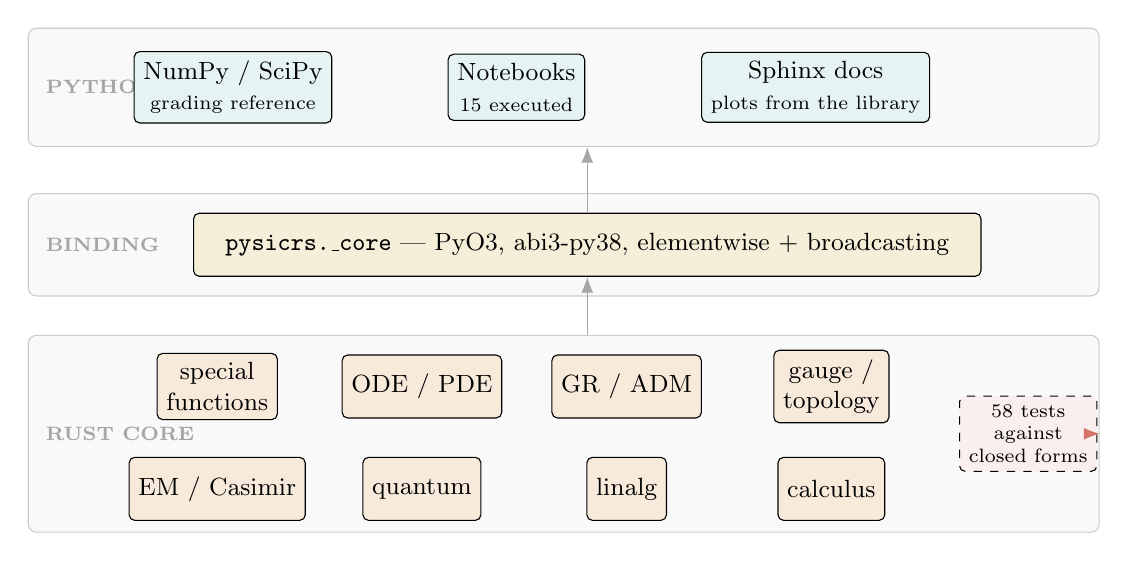
\begin{tikzpicture}[
  font=\small,
  box/.style={draw, rounded corners=2pt, minimum height=8mm, align=center, fill=white},
  lane/.style={draw=gray!40, fill=gray!5, rounded corners=3pt},
  arr/.style={-{Latex[length=2mm]}, gray!70},
]
\node[lane, minimum width=13.6cm, minimum height=1.5cm] (l1) at (0,0) {};
\node[anchor=west, gray!70, font=\scriptsize\bfseries] at ([xshift=3pt]l1.west) {PYTHON};
\node[box, fill=teal!12] (np) at (-4.2,0) {NumPy / SciPy\\\scriptsize grading reference};
\node[box, fill=teal!12] (nb) at (-0.6,0) {Notebooks\\\scriptsize 15 executed};
\node[box, fill=teal!12] (doc) at (3.2,0) {Sphinx docs\\\scriptsize plots from the library};

\node[lane, minimum width=13.6cm, minimum height=1.3cm] (l2) at (0,-2.0) {};
\node[anchor=west, gray!70, font=\scriptsize\bfseries] at ([xshift=3pt]l2.west) {BINDING};
\node[box, fill=gold!18, minimum width=10cm] (pyo3) at (0.3,-2.0)
  {\texttt{pysicrs.\_core} --- PyO3, abi3-py38, elementwise + broadcasting};

\node[lane, minimum width=13.6cm, minimum height=2.5cm] (l3) at (0,-4.4) {};
\node[anchor=west, gray!70, font=\scriptsize\bfseries] at ([xshift=3pt]l3.west) {RUST CORE};
\node[box, fill=rustorange!14] (sf) at (-4.4,-3.8) {special\\functions};
\node[box, fill=rustorange!14] (ode) at (-1.8,-3.8) {ODE / PDE};
\node[box, fill=rustorange!14] (gr) at (0.8,-3.8) {GR / ADM};
\node[box, fill=rustorange!14] (gt) at (3.4,-3.8) {gauge /\\topology};
\node[box, fill=rustorange!14] (em) at (-4.4,-5.1) {EM / Casimir};
\node[box, fill=rustorange!14] (qm) at (-1.8,-5.1) {quantum};
\node[box, fill=rustorange!14] (la) at (0.8,-5.1) {linalg};
\node[box, fill=rustorange!14] (ca) at (3.4,-5.1) {calculus};

\draw[arr] (pyo3) -- (l1.south-|pyo3);
\draw[arr] (l3.north-|pyo3) -- (pyo3);
\node[draw, dashed, rounded corners=2pt, fill=softred!8, font=\scriptsize, align=center]
  (test) at (5.9,-4.4) {58 tests\\against\\closed forms};
\draw[arr, softred!70, dashed] (test) -- (l3.east|-test);
\end{tikzpicture}
\caption{Layering. The grading reference (NumPy/SciPy) sits strictly outside the
library, so a shared bug cannot mask itself. The test plane addresses the Rust
core directly and does not go through Python.}
\label{fig:arch}
\end{figure}

\subsection{Binding surface}

Scalar functions are elementwise and shape-preserving: a float returns a float,
any sequence --- list, tuple, NumPy array --- returns a list. Two-argument
functions broadcast, and a length mismatch raises rather than truncating.

\begin{lstlisting}[language=Python]
import numpy as np, pysicrs as ps

x = np.linspace(0.1, 25, 800)
ps.bessel_j0(x)        # -> list[float], one per grid point
ps.bessel_j0(2.5)      # -> float
ps.beta(x, 2.0)        # scalar broadcasts against the sequence
\end{lstlisting}

\begin{remark}
This uniformity is not cosmetic. Two of the eighteen special functions
originally accepted only scalars, which forced a Python-level loop in exactly
the place --- plotting the function over a grid --- where a reader is most likely
to notice that the curve is wrong. Awkward interfaces suppress the checks that
would catch bugs.
\end{remark}

% =====================================================================
\section{Validation discipline}\label{sec:validation}

\begin{definition}[Graded routine]
A routine is \emph{graded} if its output is compared, over a dense sample of its
domain, against a quantity known independently of the routine: a closed form, a
tabulated value, a conserved invariant, or an established external library.
\end{definition}

The emphasis is on \emph{independently}. Three classes of invariant do most of
the work, and they are cheap because the physics supplies them.

\paragraph{Unitarity.} Any propagator built as a product of exponentials of
Hermitian operators is unitary, so $\int|\psi|^2$ is an exact invariant of the
\emph{discrete} scheme --- not merely to truncation order. This is a binary test
with no tolerance tuning: either the norm holds to round-off or the operator is
wrong.

\paragraph{Vanishing on a known solution.} Schwarzschild is a vacuum solution,
so its Ricci scalar is identically zero at every radius and every polar angle.
Any non-zero result is a defect, with no discretisation excuse available beyond
the finite-difference residual.

\paragraph{Integrality.} Topological invariants are integers. A winding number
that returns $2.9997$ is not imprecise; it is broken.

\begin{lesson}
The three properties above share a feature: they are \emph{falsifiable without
knowing the answer}. One need not know what $\psi(x,t)$ is to know that its norm
must not change. Structural invariants are the cheapest tests to write and the
hardest to satisfy by accident.
\end{lesson}

% =====================================================================
\section{Physics and the invariants it supplies}\label{sec:physics}

\subsection{Schr\"odinger and the asymmetry that forced Dirac}

The Schr\"odinger equation is first order in $t$ and second order in $\bm x$;
under a boost those derivatives transform differently, so it cannot be
covariant. This is the defect that sent Dirac looking for an alternative.

Writing $\hat H=\hat T+\hat V$ with $\hat T$ diagonal in momentum space and
$\hat V$ in position space, Strang splitting gives
\begin{equation}
e^{-i\hat H\Delta t/\hbar}
= e^{-i\hat V\Delta t/2\hbar}\,e^{-i\hat T\Delta t/\hbar}\,e^{-i\hat V\Delta t/2\hbar}
+ \mathcal O(\Delta t^3),
\end{equation}
each factor unitary. For $V=0$ a Gaussian stays Gaussian with
$\sigma(t)=\sigma_0\sqrt{1+(\hbar t/m\sigma_0^2)^2}$, which the implementation
reproduces to $1.6\times10^{-14}$.

The stationary problem discretises to a symmetric tridiagonal matrix whose
spectrum, for flat $V$, is exactly
\begin{equation}
E_k=\frac{2\hbar^2}{m\Delta x^2}\sin^2\!\Big(\frac{k\pi}{2(N+1)}\Big).
\end{equation}

\begin{figure}[h]
\centering
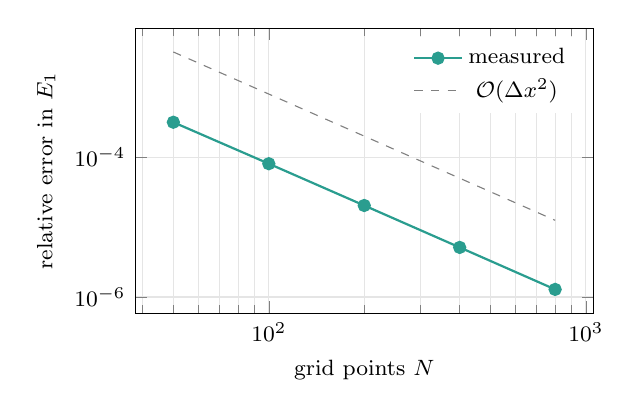
\begin{tikzpicture}
\begin{loglogaxis}[width=7.4cm,height=5.2cm,
  xlabel={grid points $N$}, ylabel={relative error in $E_1$},
  grid=both, grid style={gray!20}, tick label style={font=\footnotesize},
  label style={font=\footnotesize}, legend style={font=\footnotesize, draw=none},
  legend pos=north east]
\addplot[teal, mark=*, thick] coordinates {\databoxconv};
\addlegendentry{measured}
\addplot[gray, dashed, domain=50:800, samples=2] {8.0/(x*x)};
\addlegendentry{$\mathcal O(\Delta x^2)$}
\end{loglogaxis}
\end{tikzpicture}
\hfill
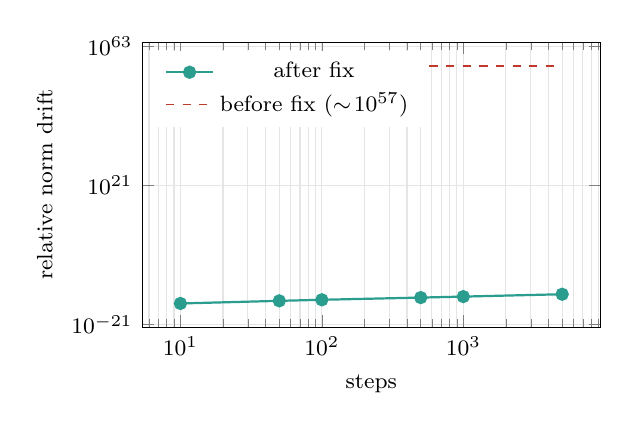
\begin{tikzpicture}
\begin{loglogaxis}[width=7.4cm,height=5.2cm,
  xlabel={steps}, ylabel={relative norm drift},
  grid=both, grid style={gray!20}, tick label style={font=\footnotesize},
  label style={font=\footnotesize}, legend style={font=\footnotesize, draw=none},
  legend pos=north west]
\addplot[teal, mark=*, thick] coordinates {\datadiracnorm};
\addlegendentry{after fix}
\addplot[softred, dashed, domain=10:5000, samples=2] {1e57};
\addlegendentry{before fix ($\sim\!10^{57}$)}
\end{loglogaxis}
\end{tikzpicture}
\caption{Left: the eigensolver converges at the expected second order. Right:
Dirac norm drift grows linearly with step count, as accumulated round-off
should. The dashed line marks where the same computation landed before the
mass-rotation defect was corrected --- note that it is off the top of any
sensible axis.}
\label{fig:convergence}
\end{figure}

\subsection{Dirac, and why unitarity is the whole test}

Requiring first-order derivatives in both $t$ and $\bm x$, together with
$E^2=p^2c^2+m^2c^4$ on iteration, forces the Clifford algebra
\begin{equation}
\{\gamma^\mu,\gamma^\nu\}=2\eta^{\mu\nu}\mathbb 1 .
\end{equation}
Numbers commute, so the coefficients must be matrices and $\psi$ a spinor. Spin
$\tfrac12$ and a negative-energy branch follow as consequences, not postulates;
the latter is antimatter.

In $1{+}1$ dimensions with $\alpha=\sigma_z$, $\beta=\sigma_x$, the mass factor
of the split-step propagator is the rotation
\begin{equation}
e^{-i\sigma_x\theta/2}=\cos\tfrac{\theta}{2}\,\mathbb 1-i\sin\tfrac{\theta}{2}\,\sigma_x,
\qquad \theta=\frac{mc^2\Delta t}{\hbar}.
\label{eq:massrot}
\end{equation}

\subsection{Zitterbewegung as a closed form}

At $p=0$ the Hamiltonian reduces to $mc^2\sigma_x$ and the evolution is exactly
solvable:
\begin{equation}
\psi(t)=\begin{pmatrix}\cos(mc^2t/\hbar)\\ -i\sin(mc^2t/\hbar)\end{pmatrix}
\ \Longrightarrow\
|\psi_R(t)|^2=\frac{1-\cos(2mc^2t/\hbar)}{2},
\end{equation}
a beat at the Compton frequency $\omega_{\rm zb}=2mc^2/\hbar$ --- matter and
antimatter interfering within one packet.

\begin{pitfall}
Our first measurement of $\omega_{\rm zb}$ integrated to $t=1.2$ when the period
is $\pi$: less than half a cycle. The FFT returned a frequency wrong by
$160\%$, with no error and no warning. A correct solver is no protection against
an incorrect measurement protocol, and a spectral estimate must always be
reported beside its resolution $2\pi/T$.
\end{pitfall}

\subsection{Aharonov--Bohm: integrality as a test}

An electron encircling a solenoid acquires $\Delta\varphi=q\Phi/\hbar$ though
$\bm B=0$ along its entire path. The observable is a geometric phase, and the
associated invariant is an integer. The implementation returns the winding of
$e^{in\theta}$ as exactly $n$ for $n=\pm1,\pm2,\pm3$, and the Berry phase of an
equatorial spinor loop as $-\pi$ to $10^{-10}$.

\subsection{ADM: gravity as a constrained system}

The $3{+}1$ split yields six evolution equations and four constraints carrying
no time derivative:
\begin{align}
\mathcal H &= {}^{(3)}\!R+K^2-K_{ij}K^{ij}-16\pi\rho = 0,\\
\mathcal M^i &= D_j\big(K^{ij}-\gamma^{ij}K\big)-8\pi j^i = 0 .
\end{align}
The total Hamiltonian of general relativity \emph{is} a constraint. On a flat
slice with $K_{ij}=c\,\delta_{ij}$ one has $\mathcal H=9c^2-3c^2=6c^2$ exactly.

\begin{figure}[h]
\centering
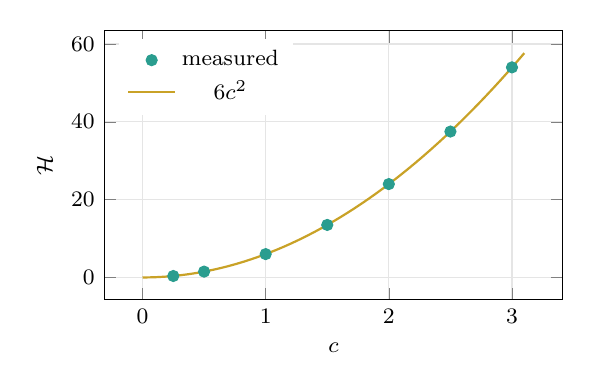
\begin{tikzpicture}
\begin{axis}[width=7.4cm,height=5cm,
  xlabel={$c$}, ylabel={$\mathcal H$}, grid=both, grid style={gray!20},
  tick label style={font=\footnotesize}, label style={font=\footnotesize},
  legend style={font=\footnotesize, draw=none}, legend pos=north west]
\addplot[only marks, mark=*, teal] coordinates {\dataadmH};
\addlegendentry{measured}
\addplot[gold, thick, domain=0:3.1, samples=50] {6*x^2};
\addlegendentry{$6c^2$}
\end{axis}
\end{tikzpicture}
\hfill
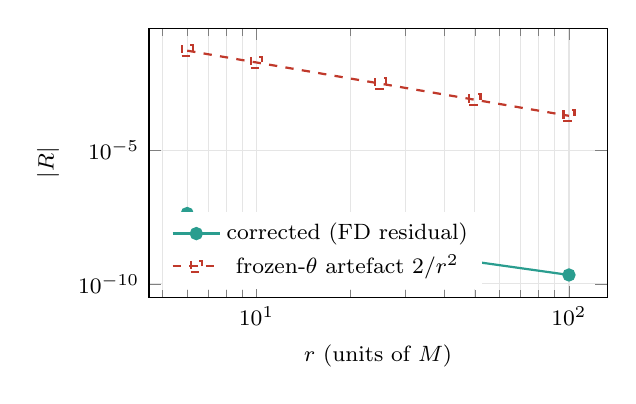
\begin{tikzpicture}
\begin{loglogaxis}[width=7.4cm,height=5cm,
  xlabel={$r$ (units of $M$)}, ylabel={$|R|$}, grid=both, grid style={gray!20},
  tick label style={font=\footnotesize}, label style={font=\footnotesize},
  legend style={font=\footnotesize, draw=none}, legend pos=south west]
\addplot[teal, mark=*, thick] coordinates {\dataricci};
\addlegendentry{corrected (FD residual)}
\addplot[softred, dashed, mark=square, thick] coordinates {\dataricciold};
\addlegendentry{frozen-$\theta$ artefact $2/r^2$}
\end{loglogaxis}
\end{tikzpicture}
\caption{Left: the Hamiltonian constraint lands on $6c^2$ with zero deviation.
Right: Schwarzschild Ricci scalar. A vacuum solution must give exactly zero; the
dashed curve is what a metric frozen at $\theta=\pi/2$ produces once
differentiated.}
\label{fig:adm}
\end{figure}

\subsection{Wheeler--DeWitt and the disappearance of time}

Quantising the constraint gives $\hat{\mathcal H}\Psi=0$, an equation with no
time derivative at all. In minisuperspace,
\begin{equation}
\frac{d^2\Psi}{da^2}+\frac{p}{a}\frac{d\Psi}{da}-U(a)\Psi=0,
\qquad U(a)=a^2-\frac{\Lambda}{3}a^4,
\end{equation}
with a turning point at $a_t=\sqrt{3/\Lambda}$. Since
$U'(a_t)=-2\sqrt{3/\Lambda}$, the substitution
\begin{equation}
z=-\big[2\sqrt{3/\Lambda}\,\big]^{1/3}(a-a_t)
\end{equation}
reduces the equation to $\Psi_{zz}=z\Psi$: the Airy equation. This converts an
otherwise ungradable problem into one with an external reference.

% =====================================================================
\section{Eight defects, and why the tests missed them}\label{sec:bugs}

Table~\ref{tab:bugs} summarises. We then analyse the failure of the tests,
which we consider the more useful result.

\begin{table}[h]
\centering\footnotesize
\begin{tabular}{@{}p{3.45cm}p{3.5cm}p{7.15cm}@{}}
\toprule
\textbf{Routine} & \textbf{Symptom} & \textbf{Cause} \\
\midrule
\texttt{dirac\_split\_step\_1d} & norm $1.77\to3.6\times10^{57}$, independent of $\Delta t$ &
  \eqref{eq:massrot} coded as $\exp(i\sin\tfrac\theta2)$ --- modulus $1$ --- instead of $i\sin\tfrac\theta2$; the step matrix becomes $\approx\left(\begin{smallmatrix}1&-1\\-1&1\end{smallmatrix}\right)$, singular values $2$ and $0$ \\[2pt]
\texttt{schrodinger\_eigen\_1d} & $32771$ where $4.93$ expected &
  Jacobi sweep with a malformed rotation angle and self-referential off-diagonal updates; returned the matrix diagonal, which scales as $1/\Delta x^2$ \\[2pt]
\texttt{rk45\_solve} & returned \texttt{None} &
  \texttt{Ok(py.None())} behind a \texttt{TODO}; the error estimator also used non-Dormand--Prince weights and applied component $[0]$ to every component \\[2pt]
\texttt{ricci\_scalar} & $R=-2/r^2$ in vacuum &
  metric froze $g_{\varphi\varphi}=r^2$ at $\theta=\pi/2$, so $\partial_\theta g_{\varphi\varphi}=0$ and the angular terms stopped cancelling \\[2pt]
\texttt{bessel\_j0/j1/y0/y1} & $J_0(7.98)=+50.6$ for $|J_0|\le1$ &
  four-term Taylor series used to $|x|=8$; asymptotic branch applied \texttt{.sin()} to the coefficient polynomial rather than the phase \\[2pt]
\texttt{airy\_ai} & \texttt{NaN} at $x=0$ &
  large-$|x|$ asymptotic applied for all $x\ge-1$, including $\xi=0$ \\[2pt]
\texttt{expint\_en} & wrong for all $n>1$ &
  computed $e^{-(k-1)}$ where $e^{-x}$ was meant \\[2pt]
\texttt{zeta} & $\zeta(2)$ to four digits; $\zeta(-1)$ wrong &
  $+N^{-s}/2$ where $-N^{-s}/2$ was needed; rising factorial built from $\lfloor s\rfloor$; reflection used \texttt{powi(s as i32)}, truncating $s$ \\
\bottomrule
\end{tabular}
\caption{The eight defects. All compiled cleanly and returned finite values.}
\label{tab:bugs}
\end{table}

\subsection{The vacuous test}

The most instructive case had a test. It read, in essence:

\begin{lstlisting}[language=Rust]
let rs = |_c: &[f64]| schwarzschild_metric(10.0, 1.0);   // ignores _c
let r = ricci_scalar(&rs, &[0.0, 10.0, FRAC_PI_2, 0.0], 1e-4);
assert!(r.abs() < 0.1);
\end{lstlisting}

The closure ignores its coordinate argument. \texttt{ricci\_scalar}
differentiates the metric it is given, so every derivative of a constant is
zero, $R$ vanishes identically, and the assertion holds for \emph{any}
implementation --- including one returning zero unconditionally. The tolerance
compounds it: $0.1$ would have admitted the $-0.02$ artefact even had the
closure been correct.

\begin{lesson}
A test that cannot fail is worse than no test, because it converts absence of
evidence into apparent evidence of absence. Before trusting an assertion, ask
what the routine would have to do to violate it. If the answer is ``nothing
plausible'', the test is measuring the harness.
\end{lesson}

\subsection{Tolerances chosen for convenience}

Several accuracy claims in the documentation were round numbers rather than
measurements: $\operatorname{erf}$ was listed at $10^{-14}$ though it implements
a formula accurate to $1.5\times10^{-7}$ \emph{by construction}; $\zeta$ at
$10^{-10}$ though it measured $1.3\times10^{-3}$. A tolerance should be derived
from the method's error term, not chosen so the test passes.

\subsection{Why $\Delta t$-independence was the tell}

The Dirac defect is worth isolating. Norm growth in a PDE solver is usually read
as instability, prompting a smaller step. Here the final norm was identical for
$\Delta t=10^{-3}$ and $10^{-5}$. An unstable scheme improves as $\Delta t$
shrinks; a \emph{non-unitary operator} does not, because the error is in the
operator rather than in the discretisation of time.

\begin{lesson}
Sweep $\Delta t$ before diagnosing instability. If the error is invariant under
the sweep, the defect is algebraic, and no step-size control will rescue it.
\end{lesson}

\subsection{Distinguishing library defects from user error}

Not all the failures were in the library. The companion notebook's Dirac cell
packed the spinor as two concatenated blocks when the binding expects
interleaved $(\psi_L,\psi_R)$ pairs, and separately multiplied the reference
norm by two ``for two components''. Another cell asserted that a wavepacket
released outside an attractive well should end up bound with probability
$\approx1$ --- which no unitary evolution can produce, since binding requires
shedding energy. Both produced anomalies that looked like solver defects.

\begin{lesson}
Before reporting a numerical bug, verify that the invariant being tested is one
the physics actually implies. Roughly a quarter of our ``findings'' were
incorrect expectations.
\end{lesson}

% =====================================================================
\section{Measured accuracy}\label{sec:accuracy}

\begin{table}[h]
\centering\footnotesize
\begin{tabular}{@{}llrll@{}}
\toprule
\textbf{Function} & \textbf{Domain} & \textbf{Error} & & \textbf{Method}\\
\midrule
$\Gamma(x)$ & $(0,100]$ & $7\times10^{-14}$ & rel. & Lanczos\\
$\ln\Gamma(x)$ & $(0,170]$ & $3\times10^{-13}$ & rel. & Lanczos\\
$B(a,b)$ & $a,b\in[0.3,8]$ & $1\times10^{-14}$ & rel. & via $\Gamma$\\
$\operatorname{erf},\operatorname{erfc}$ & $[-6,6]$ & $1\times10^{-7}$ & abs. & A\&S 7.1.26\\
$J_0,J_1$ & $[-30,30]$ & $5\times10^{-9}$ & abs. & A\&S 9.4\\
$Y_0,Y_1$ & $(0,30]$ & $2\times10^{-8}$ & abs. & A\&S 9.4\\
$P_\ell,P_\ell^m$ & $[-1,1]$ & $6\times10^{-15}$ & abs. & recurrence\\
$T_n,U_n$ & $[-1,1]$ & $3\times10^{-15}$ & abs. & recurrence\\
$\mathrm{Ai}(x)$ & $[-15,10]$ & $1\times10^{-7}$ & abs. & series + asymptotic\\
$E_n(x)$, $n\le6$ & $(0,20]$ & $1\times10^{-14}$ & rel. & series + Lentz CF\\
$\zeta(s)$ & $(1,30]$ & $2\times10^{-15}$ & rel. & Euler--Maclaurin\\
\bottomrule
\end{tabular}
\caption{Measured against SciPy on a dense grid. Two entries are limited by
their formula rather than the port: A\&S 7.1.26 is $1.5\times10^{-7}$ by
construction, and $\mathrm{Ai}$ is machine-precision on $|x|\le9$ where the
series is used, the quoted figure coming from the asymptotic branch beyond.}
\label{tab:accuracy}
\end{table}

\begin{figure}[h]
\centering
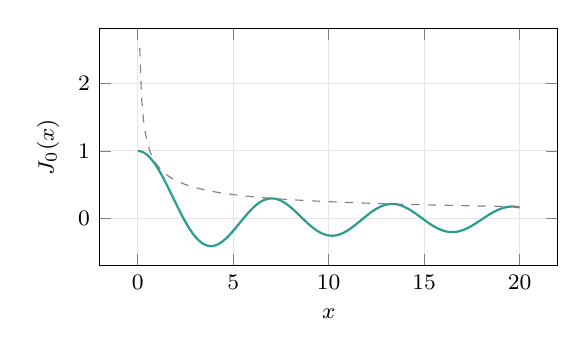
\begin{tikzpicture}
\begin{axis}[width=7.4cm,height=4.6cm, xlabel={$x$}, ylabel={$J_0(x)$},
  grid=both, grid style={gray!20}, tick label style={font=\footnotesize},
  label style={font=\footnotesize}, legend style={font=\footnotesize,draw=none}]
\addplot[teal, thick] coordinates {\databesseljzero};
\addplot[gray, dashed] coordinates {\databesselenv};
\end{axis}
\end{tikzpicture}
\hfill
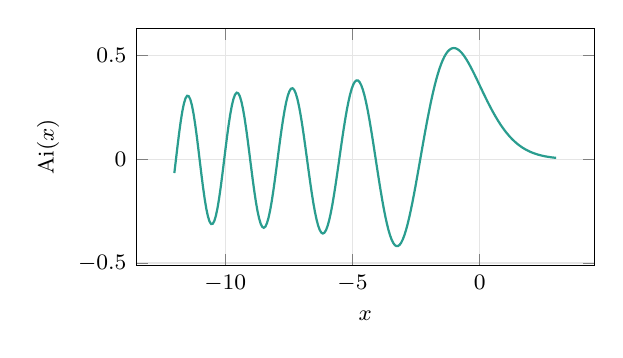
\begin{tikzpicture}
\begin{axis}[width=7.4cm,height=4.6cm, xlabel={$x$}, ylabel={$\mathrm{Ai}(x)$},
  grid=both, grid style={gray!20}, tick label style={font=\footnotesize},
  label style={font=\footnotesize}]
\addplot[teal, thick] coordinates {\dataairy};
\end{axis}
\end{tikzpicture}
\caption{$J_0$ with its $\pm\sqrt{2/\pi x}$ envelope, and $\mathrm{Ai}$ across
the turning point. Both are smooth through the internal branch switches
(at $|x|=8$ and $|x|=9$ respectively) --- the discontinuity such a switch can
introduce is itself worth testing for.}
\end{figure}

% =====================================================================
\section{Related work}

General-purpose scientific stacks (SciPy \citep{scipy2020}, GSL
\citep{gsl}) are far broader than pysic-rs and are the appropriate default.
Our contribution is not coverage but the explicit pairing of each routine with
a falsifiable reference, and the decision to publish the resulting failures.

The algorithms themselves are standard: Abramowitz \& Stegun
\citep{abramowitz1964} for the special-function approximations, Press et
al.\ \citep{numrecipes} for Dormand--Prince and the modified Lentz continued
fraction, and the EISPACK implicit QL algorithm \citep{eispack} for the
symmetric tridiagonal eigenproblem. On the physics side we follow
Dirac \citep{dirac1928}, Aharonov and Bohm \citep{ab1959}, Arnowitt, Deser and
Misner \citep{adm1959}, DeWitt \citep{dewitt1967} and Berry
\citep{berry1984}.

% =====================================================================
\section{Limitations}

pysic-rs is CPU-only and single-node; there is no GPU backend and no distributed
execution. Coverage is deliberately narrow --- the equations a graduate course
in mathematical physics actually treats --- and several modules are
one-dimensional only. \texttt{erf}/\texttt{erfc} are limited to
$1.5\times10^{-7}$ by the formula they implement, and \texttt{Ai} to $10^{-7}$
outside $|x|\le9$; both are documented rather than fixed. The
$\mathcal O(n^3)$ eigenvector accumulation makes direct diagonalisation
impractical beyond a few thousand grid points.

Most importantly, Section~\ref{sec:bugs} is a report on the routines we
examined. We have no basis for asserting that the modules not exercised by this
work are correct, and the base rate we observed --- eight defects in the
routines a single document happened to touch --- argues against optimism.

% =====================================================================
\section{Conclusion}

Rust eliminated an entire class of defects and none of the defects we actually
had. Every bug reported here was a piece of mathematics transcribed incorrectly
into code that the compiler had no way to question: a sine exponentiated instead
of multiplied, a floor applied to a real argument, a sign inverted on a
correction term.

What caught them was placing each number next to an independently known value.
That discipline is inexpensive when the physics supplies the invariant, and
unitarity, vacuum conditions and integrality supply a great many. Our
recommendation is narrow and, we think, actionable: for each routine, write down
the quantity it must preserve before writing the routine, and treat any test
that cannot fail as a defect in its own right.

\subsection*{Reproducibility}

Source, tests, notebooks and the scripts generating every figure in this paper:
\url{https://github.com/ThotDjehuty/pysic-rs}. Documentation:
\url{https://pysic-rs.readthedocs.io/}. The companion notebook
\texttt{14\_dirac\_adm\_wheeler\_dewitt.ipynb} reproduces every measured
quantity quoted here.

\begin{thebibliography}{99}\footnotesize
\bibitem[Abramowitz \& Stegun(1964)]{abramowitz1964}
M.~Abramowitz and I.~A. Stegun, \emph{Handbook of Mathematical Functions},
National Bureau of Standards, 1964.

\bibitem[Aharonov \& Bohm(1959)]{ab1959}
Y.~Aharonov and D.~Bohm, ``Significance of Electromagnetic Potentials in the
Quantum Theory'', \emph{Phys. Rev.} \textbf{115}, 485, 1959.

\bibitem[Arnowitt et al.(1959)]{adm1959}
R.~Arnowitt, S.~Deser and C.~W. Misner, ``Dynamical Structure and Definition of
Energy in General Relativity'', \emph{Phys. Rev.} \textbf{116}, 1322, 1959.

\bibitem[Berry(1984)]{berry1984}
M.~V. Berry, ``Quantal Phase Factors Accompanying Adiabatic Changes'',
\emph{Proc. R. Soc. Lond. A} \textbf{392}, 45, 1984.

\bibitem[DeWitt(1967)]{dewitt1967}
B.~S. DeWitt, ``Quantum Theory of Gravity. I. The Canonical Theory'',
\emph{Phys. Rev.} \textbf{160}, 1113, 1967.

\bibitem[Dirac(1928)]{dirac1928}
P.~A.~M. Dirac, ``The Quantum Theory of the Electron'', \emph{Proc. R. Soc.
Lond. A} \textbf{117}, 610, 1928.

\bibitem[Galassi et al.(2009)]{gsl}
M.~Galassi et al., \emph{GNU Scientific Library Reference Manual}, 3rd ed.,
Network Theory Ltd., 2009.

\bibitem[Press et al.(2007)]{numrecipes}
W.~H. Press, S.~A. Teukolsky, W.~T. Vetterling and B.~P. Flannery,
\emph{Numerical Recipes: The Art of Scientific Computing}, 3rd ed.,
Cambridge University Press, 2007.

\bibitem[Smith et al.(1976)]{eispack}
B.~T. Smith et al., \emph{Matrix Eigensystem Routines --- EISPACK Guide},
Springer, 1976.

\bibitem[Virtanen et al.(2020)]{scipy2020}
P.~Virtanen et al., ``SciPy 1.0: Fundamental Algorithms for Scientific Computing
in Python'', \emph{Nature Methods} \textbf{17}, 261, 2020.
\end{thebibliography}

\end{document}
